\chapter{Tool Evaluation}
\section{Overview/Approach}
In this section, the approach for synthesizing and generating the data will be explained in a more technical fashion.\\
As explained before, the tool is executed via a single script, this script is connected to all of the other necessary python scripts which are all contained in the same directory (excluding the external libraries).
\subsection{Connecting to the Database}
The tool uses a library called \href{https://www.psycopg.org/}{psycopg}, which is a PostgreSQL adapter for the Python programming language. It provides a level of abstraction for doing various functions with the database server. It also provides us with different features such as: Exception handling, avoiding SQL-injections, thread-safe operations, large objects support etc. Some of the features described here were very important for this tool.\\
\newline
A set of the parameters that this tool takes are database connecting parameters like: database name, host name, TCP/IP port, postgres user and that users password. With the help of these parameters, the tool, using the psycopg library, connects to the desired database server. If this connection fails because of wrong credentials or the database not existing, a message is shown on the terminal explaining the reason why the connection failed and the program is exit. All of these operations and exception handlings are done with the help of this library.\\
\newpage
Example of a connection failure:
\begin{figure}[H]
	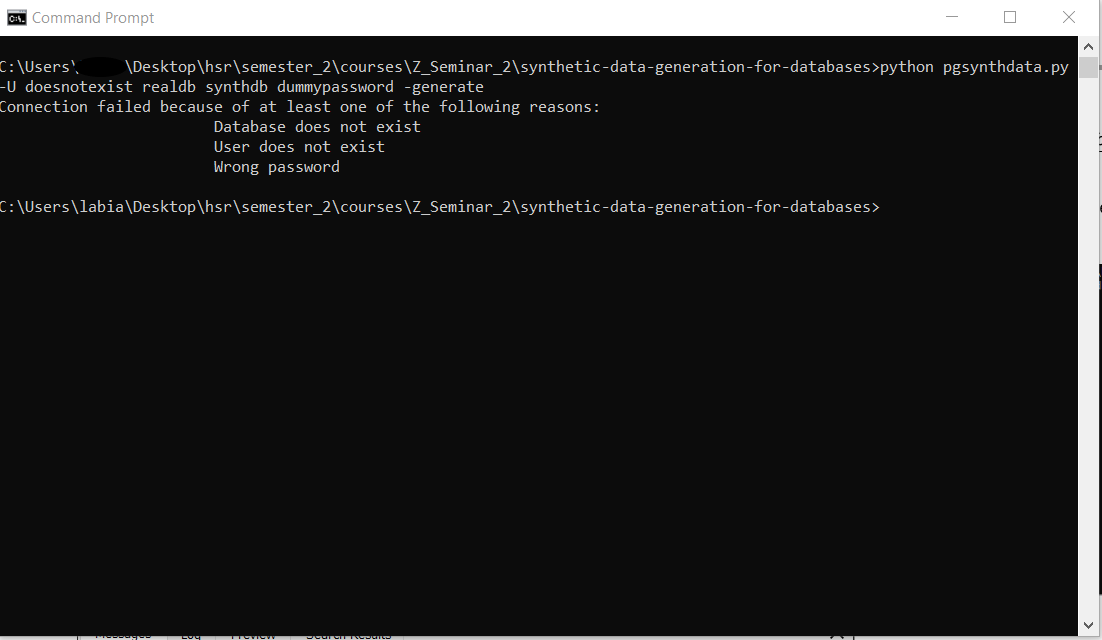
\includegraphics[width=\linewidth]{./Figures/ToolEvaluation/connection_failure_message.png}
	\caption{The message shown when the connection to the PostgreSQL database has failed}
\end{figure}
Depending on the parameters, whether \mintinline{bash}{-r} or \mintinline{bash}{--recreate} was passed, the tool either creates a new database, copying the complete schema of the primary database and leaving it empty, or it assumes that the database already exists and does not bother creating it and only connects to it.\\
The recreation is done using a combination of psycopg and shell commands that create a \textit{pg\_dump} file, specifying the connection parameters beforehand and dumping it into the same directory as the tool. After the database has been created, the \textit{pg\_dump} file is deleted from the machine because it is no longer needed.\\
\newpage
The function function that recreates the database:
\begin{minted}{python}
def copy_database_structure(args):
  print(f 'Copying the "{args.DBNAMEGEN}" database structure...')

try:
process = Popen(['pg_dump',
    '--dbname=postgresql://{}:{}@{}:{}/{}'.format(args.user,
      args.password,
      'localhost',
      '5432',
      args.DBNAMEIN),
    '-s',
    '-Fc',
    '-f', DUMP_FILE_PATH
  ],
  stdout = subprocess.PIPE)

process.communicate()[0]

process = Popen(['pg_restore',
    '--dbname=postgresql://{}:{}@{}:{}/{}'.format(args.user,
      args.password,
      'localhost',
      '5432',
      args.DBNAMEGEN),
    DUMP_FILE_PATH
  ],
  stdout = subprocess.PIPE
)

process.communicate()[0]
except Exception as error:
  sys.exit('Database structure could not be copied. Error: {}'.format(error))
finally:
if os.path.exists(DUMP_FILE_PATH):
  os.remove(DUMP_FILE_PATH)
\end{minted}
After the connection has been achieved and the database has been created/connected to, the tool proceeds with the data synthesization and generation part.\\
\subsection{Data Synthesization and Generation}
The data synthesization and generation part are the most crucial functions of this tool. They are the core logic of the tool and contain all the necessary methods for generating the synthetic data.\\
\newline
This logic of the tool is contained in a separate python script called \textit{data\_generator.py}, which contains the \textit{DataGenerator} class. This class contains all the necessary functions and attributes for generating the synthetic data.\\
It first connects to the primary database and loops through each table of the database (unless the \mintinline{bash}{-tables/--tables} parameter was supplied) and grabs information such as: primary keys, column information, pg\_stats for the table etc. It then stores this information into a huge nested dictionary, that is meant to hold such data (table names, primary keys, pg\_stats, column information). It fills only the important information and leaves the other information aside, creating a dictionary that contains only the necessary and vital statistics and numbers for the data generation.\\
\newline
After the dictionary has been fully supplied with the necessary information, another function named \textit{create\_insert\_query} is called. This function is a crucial function for the tool and it creates another sub-dictionary that contains the insert query for each table.\\
\newline
The algorithm steps for generating the data:
\begin{enumerate}
\item{Grab the important column information (data type, column name, numeric precision, numeric scale etc)}
\item{Grab information such as: the most common values and their frequencies, the average width of the column records, the factor of distinct values in the table.}
\item{Find out the number of distinct values that the tool should generate using the \textit{n\_distinct} pg\_stats value.}
\item{Since the default pg\_stats configuration stores only 100 records for the most common values and their frequencies, the numbers that their frequencies sum up to, usually does not reach 1 (unless the number of distinct values is less than 100), a dirichlet mathematical distribution is used to fill the leftover frequencies until the point that it reaches 1.\\
The Dirichlet distribution Dir(a) is a family of continuous multivariate probability distributions parameterized by a vector "a" of positive reals. It is a multivariate generalisation of the Beta distribution. Dirichlet distributions are commonly used as prior distributions in Bayesian statistics. \cite{WhatIsDirichletDistribution} \\
The dirichlet distribution is achieved in this tool with the help of the \href{https://numpy.org/}{NumPy} library.}
\item{Identify the columns data type and generate random data taken from an array of random values with weight that corresponds to the originalmost common frequencies of that column}
\item{Store all that data into a sub-dictionary that is used later for the final step of inserting the data into PostgreSQL}
\end{enumerate}
\subsection{Data Insertion}
After the synthetic data has been generated, the tool loops through each table and inserts the synthetic data into the corresponding table using the psycopg library, logging any exception or important message to the user. If an exception is thrown while inserting the data into a specific table, the transaction is rolled back and the loop moves to the next table.\\
\newline
Data insertion function snippet:
\begin{minted}[breaklines]{python}
for table_name, insert_query in insert_dict.items():
  try:
    if insert_query:
      cursor.execute(
        sql.SQL(insert_query).format(
          table_name = sql.Identifier(table_name)
        )
      ) 
      connection.commit()
  except psycopg2.DatabaseError as db_error:
    sys.stdout.write(
      f 'An error occurred while inserting data into the "{table_name}" table. Error description: {db_error}.\n')
    connection.rollback()
\end{minted}
\section{Evaluation}
TBD...
\section{Results}
TBD...